\documentclass[10pt]{article}
\usepackage[utf8]{inputenc}
\usepackage[T1]{fontenc}
\usepackage{amsmath}
\usepackage{amsfonts}
\usepackage{amssymb}
\usepackage{mhchem}
\usepackage{stmaryrd}
\usepackage{graphicx}
\usepackage[export]{adjustbox}
\graphicspath{ {./images/} }

\title{Introduction to Pumping Systems }

\author{}
\date{}


\begin{document}
\maketitle
\section{What Is In This Chapter?}
\begin{enumerate}
  \item The function of pumping systems

  \item Common pump types

  \item The basic theory of operation of centrifugal pumps

  \item The basic theory of operation of diaphragm pumps

  \item The major components of a pumping system, including the building and piping system

  \item Terms used to identify common pumps and their components

  \item The weight of a cubic foot of water

  \item How to convert between cubic feet and gallons

  \item The difference between force and pressure and what impacts them

  \item How to convert between psi and feet of head

  \item The difference between psi and feet of head

  \item The relationship between flow in cubic feet per second and gallons per minute

  \item The terms used to describe static and dynamic hydraulic conditions

  \item Headloss and its causes

  \item The terms used to describe pumping conditions

\end{enumerate}
\section{Key Words}
\begin{itemize}
  \item Amperage

  \item Axial Flow Pumps

  \item Can Turbine Pumps

  \item Cavitation

  \item Centrifugal Force

  \item Centrifugal Pump

  \item Close-coupled Pumps

  \item Concentric Reducer

  \item Displacement Pumps

  \item Dynamic Pumps - Eccentric Reducer

  \item End Suction Centrifugal

\end{itemize}
Pumps

\begin{itemize}
  \item Energy

  \item Foot Valve

  \item Force

  \item Frame-mounted Pumps

  \item Headloss

  \item Horsepower

  \item Impeller - Inertia

  \item Line Shaft Turbine Pumps

  \item Mechanical Seal

  \item Packing

  \item Pressure

  \item Pump Bowl

  \item Seal Water

  \item Shroud

  \item Split Case Pumps - Static

  \item Stuffing Box

  \item Submersible Turbine Pumps

  \item Suction Head

  \item Suction Lift

  \item Total Dynamic Head

  \item Velocity Head

  \item Vertical Turbine Pumps

  \item Volute

\end{itemize}
\section{Lesson Content}
This lesson provides an overview of the major pumping-related components found in small water systems. The lesson focuses on descriptions of components, common names, and general function.

\section{Pump Stations}
\section{Functions}
Pumping stations in small communities are used for the following purposes:

\begin{itemize}
  \item Remove water from a source, such as a river, lake, reservoir, well, spring, or muskeg pond.

  \item Move water from the treatment plant to the distribution system or reservoir.

  \item Circulate water through a distribution system.

  \item Maintain pressure in the distribution system.

  \item Circulate glycol through a heat exchanger or heating loop.

  \item Pump chemicals into the system.

\end{itemize}
\section{Major Components}
A pump station is composed of four sets of components:

\begin{itemize}
  \item The building

  \item The hydraulic system: the pump and related piping

  \item The electrical system: the motor and its related components

  \item The control system: pressure, flow, and level switches

\end{itemize}
\section{Pump Station Buildings}
\section{Introduction}
In medium-to-large facilities, pumping stations are usually separate buildings. In small systems, while they can be separate buildings, they are normally associated with the treatment plant, watering point, or other buildings.

\section{Basic Consideration}
Regardless of the design, most pumping station buildings are designed with the door opening out to allow access should there be a broken water line in the building. In addition, the buildings should be vandal-resistant, well-heated in the winter, and properly vented in the summer.

\section{Hydraulic System}
\section{Pump Types}
The pumps used in small water systems can be divided into two general categories. The basic difference between the two types is their response to changes in discharge pressure.

'Dynamic Pumps - Pumps in which the energy is added to the water continuously and the water is not contained in a set volume.

${ }^{2}$ Displacement Pumps - Pumps in which the energy is added to the water periodically and the water is contained in a set volume. - Dynamic pumps ${ }^{1}$ - Dynamic pumps are used in conditions where high volumes are required and a change in flow is not a problem. As the discharge pressure on a dynamic pump is increased, the quantity of water pumped is reduced. One type of dynamic pump, centrifugal pumps, are the most common pump used in water systems. Dynamic pumps can be operated for short periods of time with the discharge valve closed.

\begin{itemize}
  \item Displacement pumps ${ }^{2}$ - Displacement pumps are used in conditions where relatively small, but precise, volumes are required. Displacement pumps will not change their volume with a change in discharge pressure. Displacement pumps are also called positive displacement pumps. The most common positive displacement pump is the diaphragm pump used to pump chlorine and fluoride solutions. Operating a displacement pump with the discharge valve closed will damage the pump.
\end{itemize}
\includegraphics[max width=\textwidth]{2022_11_03_65aa625ded296bdfd01fg-03}

\section{Centrifugal Pumps - Pumping Theory}
\section{Energy Input Device}
A pump is a device that puts energy ${ }^{3}$ into the water. This energy can be expressed in two ways: an increase in pressure or an increase in flow.

\section{Centrifugal Pumps - Energy Input}
If you were to cut a section out of the top of a pipe and use a canoe paddle to move the water, you would have a pump. It would not be very efficient, but you would be inputting energy into the water. If you reshaped the paddle into an impeller ${ }^{4}$, you would be able to place more energy into the water. The energy would be transferred from the impeller to the water due to the friction between the impeller and the water. However, water would splash out onto the floor. This is because centrifugal force ${ }^{5}$ causes the water to fly outward away from the impeller.

\section{The Pump Case}
If you surrounded the impeller with a case, you could control the water and obtain a more efficient energy transfer. The case that you would use is volute (spiral-shaped). Volute ${ }^{6}$ is a geometrical shape, like a circle or a square. For example, a snail shell is volute-shaped. The shape of the case helps to determine the direction of rotation of the pump.

\includegraphics[max width=\textwidth]{2022_11_03_65aa625ded296bdfd01fg-03(1)}

${ }^{3}$ Energy - The ability to do work. Energy can exist in several different forms, such as heat, light, mechanical, electrical, or chemical. Energy can neither be created nor destroyed, but can be transferred from one form to another. Energy exists in one of two states: potential or kinetic.

${ }^{4}$ Impeller $-$ A rotating set of vanes designed to impart rotation to a mass of fluid.

${ }^{5}$ Centrifugal force - The force that when a ball is whirled on a string, pulls the ball outward. On a centrifugal pump, it is the force that throws water from the spinning impeller.

${ }^{6}$ Volute - The spiral-shaped casing surrounding a pump impeller that collects the liquid discharged by the impeller.

\section{Pump Rotation}
The direction of rotation can be determined when looking into the suction side of the volute case. For example, in the case below, the direction of rotation is counterclockwise.\\

\includegraphics[max width=\textwidth]{2022_11_03_65aa625ded296bdfd01fg-04}

${ }^{7}$ Centrifugal Pump - A pump consisting of an impeller fixed on a rotating shaft and enclosed in a casing, and having an inlet and discharge connection. The rotating impeller creates pressure in the liquid by the velocity derived from centrifugal force.

In summary, there are two theories that explain how a centrifugal pump ${ }^{7}$ works:

\begin{itemize}
  \item Energy transfer - the transfer of energy from the shaft to the impeller and from the impeller to the water.

  \item Centrifugal force - the force used to throw the water from the impeller.

\end{itemize}
\section{Centrifugal Pumps Configuration}
\section{Three Different Configurations}
${ }^{8}$ End Suction Centrifugal Pumps - The most common style of centrifugal pump. The center of the suction line is centered on the impeller eye. End suction centrifugal pumps are further classified as either frame-mounted or close-coupled.

\begin{itemize}
  \item Split Case Pumps - A centrifugal pump designed so that the volute case is split horizontally. The case divides on a plane that cuts though the eye of the impeller.
\end{itemize}
${ }^{10}$ Vertical Turbine Pumps - A classification of centrifugal pumps that are primarily mounted with a vertical shaft; the motor is commonly mounted above the pump. Vertical turbine pumps are either mixed or axial flow devices.

Centrifugal pumps can be divided into one of three classifications based on their configuration: end suction centrifugal ${ }^{8}$, split case $^{9}$, and vertical turbines ${ }^{10}$.

\includegraphics[max width=\textwidth]{2022_11_03_65aa625ded296bdfd01fg-04(1)}

End suction centrifugal

\includegraphics[max width=\textwidth]{2022_11_03_65aa625ded296bdfd01fg-04(2)}

Split case

\includegraphics[max width=\textwidth]{2022_11_03_65aa625ded296bdfd01fg-04(3)}

Vertical turbine

\section{End Suction Centrifugal - Types}
The end suction centrifugal pump is the most common centrifugal pump and the one we have in mind when we think about centrifugal pumps. There are two types of end suction pumps:

\begin{itemize}
  \item Close-coupled ${ }^{11}-$ A close-coupled pump has only one shaft and one set of bearings: the motor shaft and bearings. The pump impeller is placed directly onto the motor shaft. Close-coupled pumps require less space and are less expensive than frame-mounted pumps.\\

\includegraphics[max width=\textwidth]{2022_11_03_65aa625ded296bdfd01fg-05}

  \item Frame-mounted ${ }^{12}$ - A frame-mounted pump has a shaft and bearings separate from the motor. A coupling is required to get the energy from the motor to the pump.\\

\includegraphics[max width=\textwidth]{2022_11_03_65aa625ded296bdfd01fg-05(1)}

\end{itemize}
For safety purposes, couplings should have guards installed.

\section{Split Case Pumps}
Split case pumps are unique. The case has a row of bolts that allow half of the case to be removed, providing access to the entire rotating assembly for inspection or removal. These pumps are normally found as fire service pumps and circulation pumps in medium-to-large communities. The circulation pumps in Nome and Fairbanks are split case pumps.

\section{Vertical Turbines}
There are four styles of vertical turbines: line shaft ${ }^{13}$, axial flow $^{14}$, can turbine ${ }^{15}$ and the submersible turbine ${ }^{16}$. The vertical turbine and the submersible turbine are found in rural communities in Alaska. The primary difference between the vertical turbine and the submersible turbine is the position of the motor. The pumping assembly is the same. Submersible turbine pumps in Alaska can range from 5 gpm to 100 gpm or more. ${ }^{11}$ Close-coupled Pumps - End suction centrifugal pumps in which the pump shaft and motor shaft are the same. The pump bearings and motor bearings are also the same. The impeller is attached directly onto the end of the motor shaft. ${ }^{12}$ Frame-mounted Pumps - End suction centrifugal pumps designed so that the pump bearings and pump shaft are independent of the motor. This type of pump requires a coupling between the pump and the motor in order to transfer energy from the motor to the pump. ${ }^{13}$ Line Shaft Turbine Pumps - A type of vertical turbine. In this type of vertical turbine, the motor is mounted above the ground, and the pump unit is mounted below the water surface. A column extends from the pump to a discharge head found just below the motor. A shaft extends on a straight line from the center of the motor to the pump. The pump may be mounted a few feet to several hundred feet away from the motor.

${ }^{14}$ Axial Flow Pumps - A type of vertical turbine that uses a propeller instead of an impeller. In axial flow pumps, the energy is transferred into the water so that the direction of the flow is directly up the shaft.

${ }^{15}$ Can Turbine Pumps - A type of line shaft turbine. The pump assembly is mounted inside of a sealed can. The inlet is mounted opposite the outlet on the discharge head. The can must always be under pressure.

${ }^{16}$ Submersible Turbine Pumps - A style of vertical turbine pump in which the entire pump assembly and motor are submersed in the water. The motor is commonly mounted below the pump.

\includegraphics[max width=\textwidth]{2022_11_03_65aa625ded296bdfd01fg-06}

Axial flow turbine

\includegraphics[max width=\textwidth]{2022_11_03_65aa625ded296bdfd01fg-06(1)}

Can turbine

\includegraphics[max width=\textwidth]{2022_11_03_65aa625ded296bdfd01fg-06(2)}

Submersible turbine

\section{End suction Centrifugal and Split Case Components}
\section{Shaft and Bearings}
The shaft is used to transfer energy from the motor to the impeller. The most common shaft materials are high carbon steel and stainless steel. Each shaft is supported by bearings that support loads along the shaft, called thrust loads, and loads at right angles to the shaft, called radial loads. The bearings may or may not be part of the motor.

\section{Impellers}
${ }^{17}$ Shroud - The front and/or back of an impeller.

The energy is transferred from the shaft to the impeller and from the impeller to the water. There are three types of impellers, based on the number of shrouds ${ }^{17}$ :

\begin{itemize}
  \item Closed impeller - When an impeller has a shroud in the front and in the back.

  \item Semi-open impeller - When there is only a shroud in the back of the impeller.

  \item Open impeller - When there are no shrouds.

\end{itemize}
The impeller type is selected by the pump manufacturer to meet specific conditions.

\includegraphics[max width=\textwidth]{2022_11_03_65aa625ded296bdfd01fg-06(3)}

Closed

\includegraphics[max width=\textwidth]{2022_11_03_65aa625ded296bdfd01fg-06(4)}

Semi-open

\includegraphics[max width=\textwidth]{2022_11_03_65aa625ded296bdfd01fg-06(5)}

Open

\section{Wear Rings}
With closed impellers, the impeller fits very close to the case. As a result, the case is worn by material passing from the high-pressure side to the low-pressure side of the impeller. To protect the case, brass or stainless steel wear rings are inserted into the case.

\section{Volute Case}
Around the impeller is the volute case. The volute case gathers the water thrown from the impeller and directs it in a single direction.\\

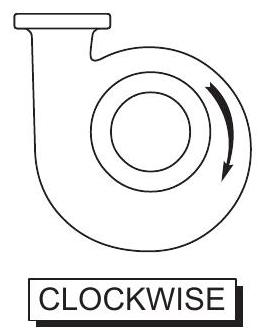
\includegraphics[max width=\textwidth]{2022_11_03_65aa625ded296bdfd01fg-07}

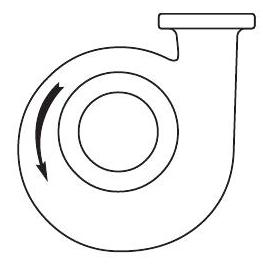
\includegraphics[max width=\textwidth]{2022_11_03_65aa625ded296bdfd01fg-07(1)}

COUNTER CLOCKWISE

\section{Backing Plate}
Behind the volute case is the backing plate. The backing plate seals the back of the volute case area.

\section{Stuffing Box}
Attached to, and sometimes part of, the backing plate is the stuffing box ${ }^{18}$. The stuffing box is where material that controls the leakage of water from around the shaft is placed. The material placed in the stuffing box is either packing ${ }^{19}$ or a mechanical seal $^{20}$.

\section{Packing/Mechanical Seals}
Packing and mechanical seals serve the same purpose: they control leakage through the stuffing box. Packing is composed of some type of fiber, like cotton, and some type of lubricant, like graphite or Teflon ${ }^{\mathrm{TM}}$. A mechanical seal is composed of two finely machined surfaces, one hard and one soft, that prevent water from passing. When installing packing, joints should be staggered.

\section{Packing Gland}
In order to control leakage with packing, pressure must be placed on the packing. This pressure is applied by the packing gland, two pieces of metal at the back of the stuffing box. There should be a slow drip from the stuffing box to show lubrication between the shaft and the packing.

\section{Lantern Ring}
It is often desirable to lubricate and cool the packing with external water or oil. When water is used, it is called seal water ${ }^{21}$ or flush water. The seal water is distributed into the stuffing box through the lantern ring, which is commonly a brass ring with holes that allow the water to easily pass.

\section{Shaft Sleeve}
To protect the shaft from damage due to the packing, a shaft sleeve can be installed. A shaft sleeve is a brass or stainless steel sleeve that fits tightly over the shaft. ${ }^{18}$ Stuffing Box - That portion of the pump that houses the packing or mechanical seal. Usually referred to as the dry portion of the pump. The stuffing box is located in back of the impeller and around the shaft.

${ }^{19}$ Packing - Material made of woven animal, plant, mineral, or metal fiber and some type of lubricant, placed in rings around the shaft of a pump and used to control the leakage from the stuffing box.

${ }^{20}$ Mechanical Seal - A mechanical device used to control leakage from the stuffing box of a pump and usually made of two flat surfaces, one of which rotates on the shaft. The two flat surfaces are of such close tolerances as to prevent the passage of water between them.

${ }^{21}$ Seal Water - The water supplied to the stuffing box to lubricate and flush the packing or the mechanical seal.

\includegraphics[max width=\textwidth]{2022_11_03_65aa625ded296bdfd01fg-08}

Stuffing box

\includegraphics[max width=\textwidth]{2022_11_03_65aa625ded296bdfd01fg-08(1)}

BRAIDED FABRIC

Packing

\includegraphics[max width=\textwidth]{2022_11_03_65aa625ded296bdfd01fg-08(2)}

Mechanical seal

\includegraphics[max width=\textwidth]{2022_11_03_65aa625ded296bdfd01fg-08(3)}

Shaft sleeve threaded to shaft

\section{Review}
\begin{enumerate}
  \item List the two major categories of pumps.

  \item How is energy transferred from the impeller of a centrifugal pump to the water?

  \item The energy placed into the water by a pump can be expressed as an increase in and an increase in

\end{enumerate}
\section{End suction Centrifugal and Split Case Piping}
\section{Suction Conditions}
End suction and split case pumps can be installed in suction lift ${ }^{22}$ or suction head ${ }^{23}$ conditions. (See Hydraulics section for a more detailed explanation.) The piping system associated with the pump varies slightly depending on the suction conditions. Since the suction lift condition is the most difficult, it is used in the following description.

\includegraphics[max width=\textwidth]{2022_11_03_65aa625ded296bdfd01fg-09}

Suction lift

\includegraphics[max width=\textwidth]{2022_11_03_65aa625ded296bdfd01fg-09(1)}

Suction head

\section{Suction Piping}
Most pumps in a suction lift condition require a foot valve $^{24}$ on the end of the suction line to prevent the pump from losing prime. Most foot valves are large globe valves. The suction piping is usually designed one pipe size larger than the inlet of the pump with smooth piping material and fittings. Isolation valves on the suction side of a pump should only be gate or ball valves. Butterfly valves cause high headloss ${ }^{25}$. As the piping reaches the pump, it is reduced to meet the pump connection using an eccentric reducer ${ }^{26}$. The eccentric reducer prevents air accumulation in the piping.

\includegraphics[max width=\textwidth]{2022_11_03_65aa625ded296bdfd01fg-09(2)}

${ }^{22}$ Suction Lift - A pumping condition where the eye of the impeller of the pump is above the surface of the water from which the pump is pumping. ${ }^{23}$ Suction Head - A pumping condition where the eye of the impeller of the pump is below the surface of the water from which the pump is pumping. ${ }^{24}$ Foot Valve - A one-way valve placed at the entrance of a suction line that is opened by the flow of water. The purpose of the valve is to prevent reverse flow.

${ }^{25}$ Headloss - The loss of energy as a result of friction, commonly expressed in feet. The loss is actually a transfer to heat.

${ }^{26}$ Eccentric Reducer - A device used to connect a large pipe to a smaller pipe so that one edge of both pipes is aligned. ${ }^{27}$ Concentric Reducer - A device used to connect a large pipe to a smaller pipe so that the center lines of both pipes are aligned. ${ }^{28}$ Pump Bowl - The case that functions as a volute case on a mixed flow vertical turbine.

\section{Discharge Piping}
The discharge side of a pump usually starts with a concentric reducer ${ }^{27}$, which takes the pipe up to one pipe size larger than the pump discharge. An isolation valve, preferably a gate or ball valve, is normally installed on the discharge. To reduce repair costs, a flange-by-flange spool or expansion joint is placed between the isolation valve and the pump.

\section{Controlling Flow and Pressure}
Ball valves and wide body globe valves are used to control flow and pressure from a pump as well as reduce water hammer during shutdown.

\section{Check Valve}
To prevent the flow of water back through the pump, a check valve is often placed in the discharge line. If there is a flow or pressure control valve, then a check valve is not necessary.

\section{Gauges}
To evaluate pump operating conditions, pressure gauges are placed on the suction and discharge sides of a pump. Ball valves are installed at the base of the gauges to allow easy replacement and to shut the gauges off when not in use, thus extending their life.

\section{Seal Water}
Seal water is usually supplied from the discharge of the volute case. If the seal water is obtained from some other source, a pressure gauge should be installed in the seal water line in order to assure that flow is in the correct direction, and backflow protection should be provided with an air gap.

\section{Vertical Turbine Components}
\section{Line Shaft and Submersible}
Vertical turbines, as discussed here, include line shaft and submersible turbines.

\section{Inlet}
Water enters the vertical turbine through the suction bell. It then passes into the pump bowl ${ }^{28}$. The bowl serves the same function as the volute case on an end suction centrifugal. This is where energy is transferred to the water by the impellers.

\section{Impellers}
Most line shaft and submersible turbines have more than one impeller. Each impeller and pump bowl is referred to as a pump stage. Adding stages increases the discharge pressure of the pump, but not its flow.

\section{Column}
Water passes out of the pump bowl assembly and into the column. In the center of the column is the pump shaft, which may be lubricated with water or oil.

\section{Discharge Head}
The large cast iron component at the top of the pump is the discharge head. It is here that the direction of flow is changed from vertical to horizontal. The discharge head also contains the stuffing box and the mechanical seal or packing. Motor

On top of the discharge head is the pump motor. The motor can be removed from the pump by removing a nut on the pump shaft located on the top of the motor. The motor can then be lifted off the pump shaft for maintenance.

\includegraphics[max width=\textwidth]{2022_11_03_65aa625ded296bdfd01fg-11}

\section{Vertical Turbine Special Piping}
\section{Reversal of Flow}
When a vertical turbine is shut down, water runs back down the column or drop line. Line shaft turbines have special non-reversing ratchets built into the motor to prevent the pump from spinning backwards. Small submersible turbines are installed with a check valve at the top of the pump to prevent water from running backwards through the pump.

Air Control

To prevent contamination from entering the discharge line through the stuffing box, an air valve is placed on the discharge line. This valve allows air in and, when the pump starts, allows the air out.

\section{Flow - Pressure Control}
Like the end suction centrifugal, flow and pressure control with vertical turbines is accomplished using wide body globe valves and butterfly valves.

\includegraphics[max width=\textwidth]{2022_11_03_65aa625ded296bdfd01fg-12}

\section{Submersible Turbine Components}
Inlet

The water inlet into a submersible turbine is between the pump and the motor. Water moves through pump bowls that are, in most cases, identical to those of the line shaft turbine.

Drop Pipe

Water moves up from the submersible turbine, through the drop pipe, and out the discharge head.

\includegraphics[max width=\textwidth]{2022_11_03_65aa625ded296bdfd01fg-12(1)}

\section{Cavitation}
Cavitation is the condition where vapor bubbles are formed in a flowing liquid when the pressure of the liquid falls below its vapor pressure. Once the bubbles reach an area where the pressure increases above vapor pressure, the bubbles collapse thereby creating small areas of high temperature and emitting shock waves.

Cavitation in a centrifugal pump occurs when the inlet pressure falls below the design inlet pressure or when the pump is operating at a flow rate higher than the design flow rate. When the inlet pressure in the flowing liquid falls below its vapor pressure, bubbles begin to form in the eye of the impeller. Once the bubbles move to an area where the pressure of the liquid increases to above its vapor pressure, the bubbles collapse thereby emitting a "shock wave." These shock waves can pit the surface of the impeller and shorten its service life. The collapse of the bubbles also emits a pinging or crackling noise that can alert the operator that cavitation is occurring.

Cavitation is undesirable because it can damage the impeller, cause noise and vibration, and decrease pump efficiency.

\section{Positive Displacement Pumps}
\section{Major Components}
While there are several different types of positive displacement pumps available, this section is limited to those commonly used in small water systems.

Never pump against a closed discharge or suction valve when using any positive displacement pump. This could result in severe damage to personnel and/or equipment.

\section{Diaphragm Pumps}
The diaphragm pump is composed of the following:

\begin{itemize}
  \item A chamber used to pump the fluid

  \item A diaphragm operated by either electric or mechanical means

  \item Two valve assemblies: a suction valve assembly and a discharge valve assembly

\end{itemize}
When the diaphragm is pulled back, a vacuum is created in the chamber in front of the diaphragm. This vacuum causes the discharge valve to be forced closed against its seat. The vacuum allows atmospheric pressure to push fluid up against the outside of the suction valve, opening the valve and filling the chamber. When pressure is returned to the diaphragm, forcing it toward the front of the chamber, the increased pressure causes the suction valve to be forced closed and the discharge valve to be forced open. The fluid is pushed out of the chamber, and the pumping cycle starts over.

\includegraphics[max width=\textwidth]{2022_11_03_65aa625ded296bdfd01fg-13}

SUCTION PHASE

\includegraphics[max width=\textwidth]{2022_11_03_65aa625ded296bdfd01fg-13(1)}

DISCHARGE PHASE

\section{Piping System}
The piping system for diaphragm pumps used to pump chemicals is relatively simple. There are a foot valve and screen on the suction line and a check valve on the end of the discharge line. The foot valve prevents loss of prime. The discharge check valve prevents the system water from flowing back into the chemical feed tank.

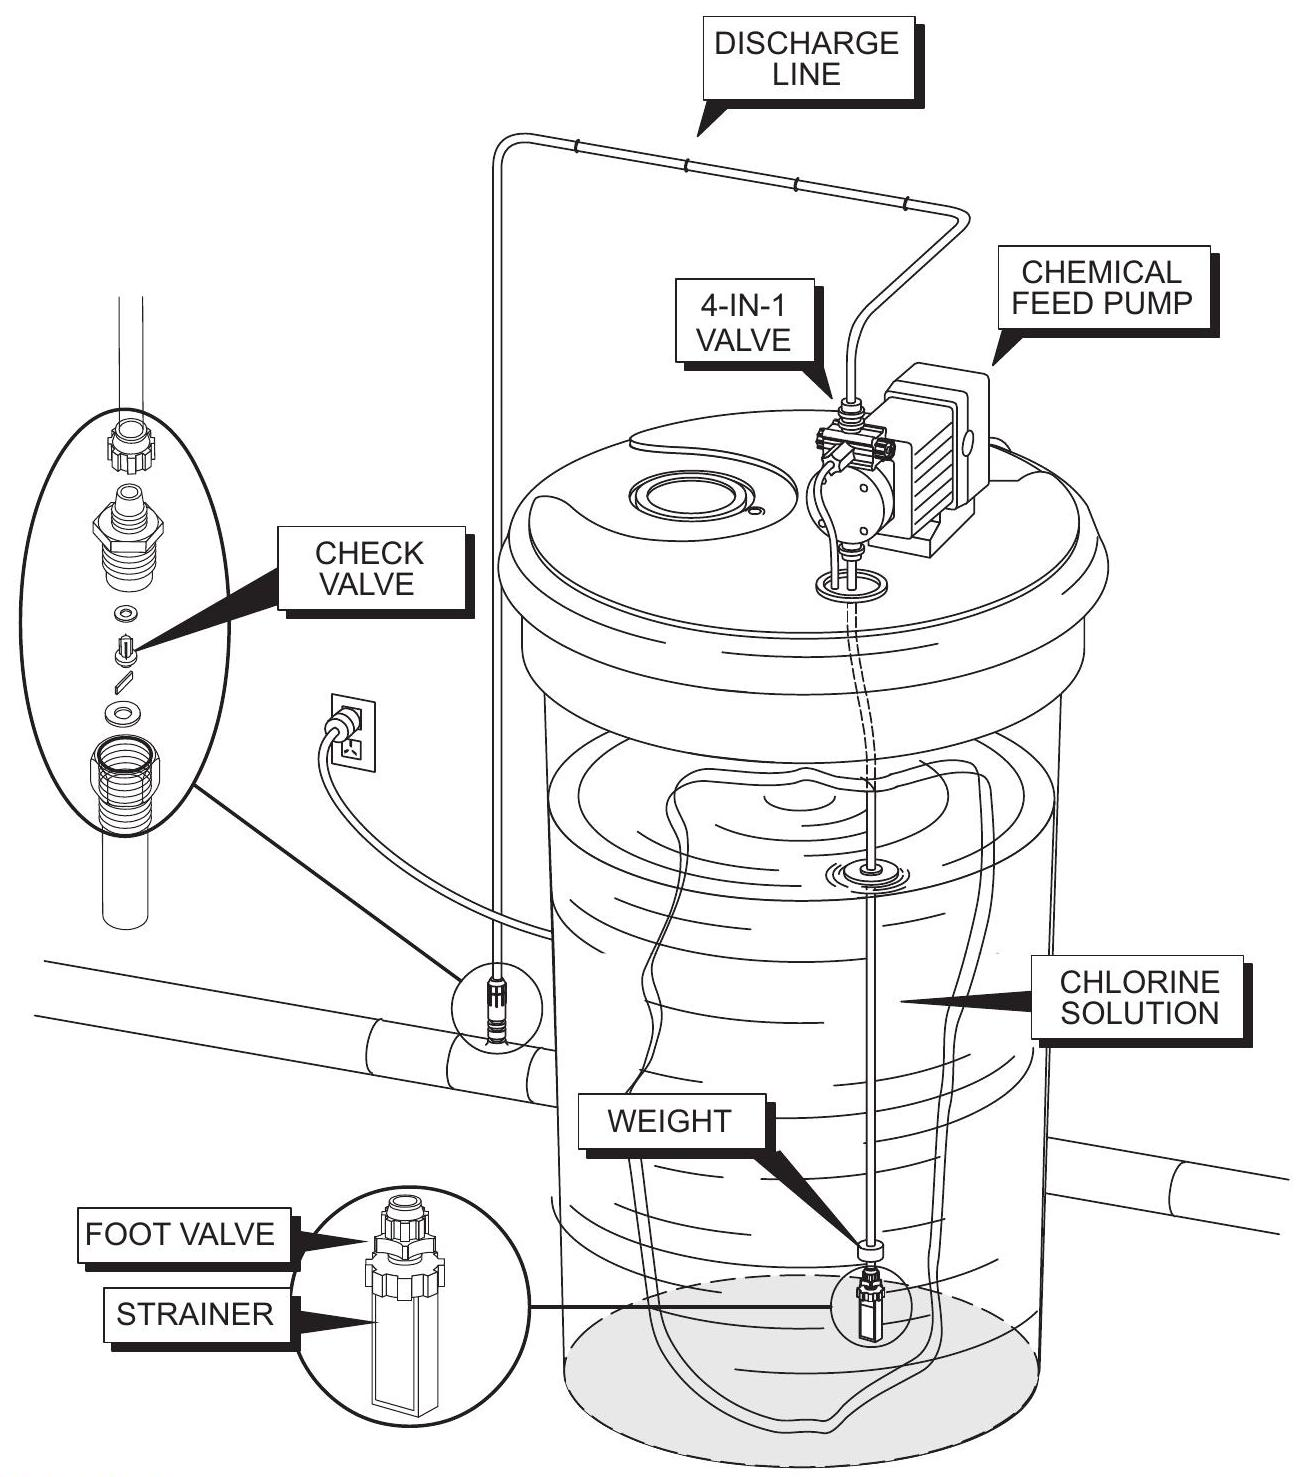
\includegraphics[max width=\textwidth]{2022_11_03_65aa625ded296bdfd01fg-14}

\section{Piping System}
\section{Peristaltic Pumps}
A peristaltic pump is a type of positive displacement pump used for pumping a variety of fluids, such as chemicals and sludges. The fluid is contained within a flexible tube fitted inside a circular pump casing. A rotor with a number of rollers (or shoes) is attached to a rotating arm that compresses the flexible tube. As the rotor turns, the part of tube under compression closes, thus forcing the fluid to be pumped through the tube. This works much like squeezing toothpaste out of a tube.

Since they have no moving parts in contact with the fluid, peristaltic pumps are inexpensive to manufacture. Their lack of valves, seals, and glands makes them comparatively inexpensive to maintain, and the use of a hose or tube makes for a relatively low-cost maintenance item compared to other pump types. It is important to select tubing with appropriate chemical resistance towards the liquid being pumped. Types of tubing commonly used in peristaltic pumps include polyvinyl chloride (PVC), silicone rubber, and fluoropolymer. Trade names include Tygon ${ }^{\mathrm{TM}}$ and Viton ${ }^{\mathrm{TM}}$.

\section{Progressive Cavity Pumps}
A progressive cavity pump moves fluid by means of a rotary screw or rotor turning within a stationary stator. The flow rate is proportional to the rotation rate of the pump. Progressive cavity pumps are designed to transfer fluid or fluids with suspended solids. They are frequently used to pump sludge, but can be used to meter large volumes of chemicals in a precise manner.

\section{Operation}
As the rotor turns, "humps" built into the rotor move within cavities in a synthetic rubber stator. This action squeezes material out of the end of the pump in much the same way as with peristaltic pumps. These pumps should always run with a fluid inside to lubricate the pump. A progressive cavity pump should never be operated against a closed valve.

\section{Basic Hydraulic Terms and Concepts}
This brief discussion on hydraulics is intended as a background necessary to understand the pumping and piping systems at a beginning level. The lesson is divided into two parts; 1) basic hydraulic terms and concepts and 2) pumping hydraulics.

\section{Weight-Volume Relationship}
\section{Weight per Cubic Foot}
Cubic feet and gallons are both used to describe a volume of water. There is a defined relationship between these two methods of measurement. The specific weight of water is defined relative to a cubic foot. One cubic foot of water weighs $62.4$ pounds. This relationship is true only at a temperature of $4^{\circ} \mathrm{C}$ and at a pressure ${ }^{29}$ of one atmosphere (called standard temperature and pressure). However, the weight varies so little that for practical purposes we use this weight from a temperature of $0^{\circ} \mathrm{C}$ to $100^{\circ} \mathrm{C}$.

29 Pressure - The force exerted on a unit area. Pressure $=$ Weight $x$ Height. In water, it is usually measured in psi (pounds per square inch). One foot of water exerts a pressure of $0.433$ pounds per square inch.

$1 \mathrm{ft}^{3} \mathrm{H}_{2} \mathrm{O}=62.4 \mathrm{lbs}$

Volume per Cubic Foot

At standard temperature and pressure, one cubic foot of water contains $7.48$ gallons. With these two relationships we can determine the weight of one gallon of water. This is accomplished by dividing the weight $(62.4 \mathrm{lbs})$ by the volume in gallons $(7.48$ gallons per cubic foot).

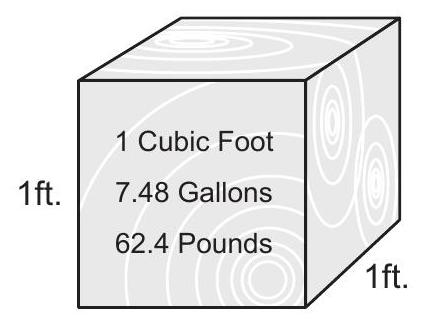
\includegraphics[max width=\textwidth]{2022_11_03_65aa625ded296bdfd01fg-15}

$1 \mathrm{ft}$. wt of gal of water $=\frac{62.4 \mathrm{lbs}}{7.48 \mathrm{gal}}=8.34 \mathrm{lbs} / \mathrm{gal}$ ${ }^{30}$ Force - Influence (as a push or pull) that causes motion. Physics - The mass of an object times its acceleration: $F$ $=$ ma. ${ }^{31}$ Head - The measure of the pressure of water expressed as height of water in feet: $1 \mathrm{psi}=2.31$ feet of head. Summary

$1 \mathrm{ft}^{3} \mathrm{H}_{2} \mathrm{O}=7.48$ gallons

1 gallon $\mathrm{H}_{2} \mathrm{O}=8.34$ pounds

Conversion $\mathrm{ft}^{3}$ to gallons

With this information we can convert cubic feet to gallons by simply multiplying the number of cubic feet by $7.48 \mathrm{gal} / \mathrm{ft}^{3}$.

\section{Example - Conversion $\mathrm{ft}^{3}$ to gallons}
Find the number of gallons in a reservoir that has a volume of $668.5 \mathrm{ft}^{3}$.

$668.5 \mathrm{ft}^{3} \times 7.48 \mathrm{gal} / \mathrm{ft}^{3}=5,000 \mathrm{gallons}$

\section{Force and Pressure}
\section{Force}
In the English system force ${ }^{30}$ and weight are often used in the same way. The weight of the cubic foot of water is $62.4$ pounds. The force exerted on the bottom of the one foot cube is $62.4$ pounds. If we have two cubes stacked on top of one another, the force on the bottom will be $124.8$ pounds.

\section{Pressure}
Pressure is a force per unit of area, pounds per square inch or pounds per square foot are common expressions of pressure. The pressure on the bottom of our cube is $62.4$ pounds per square foot. It is normal to express pressure in pounds per square inch (psi). This can be accomplished by determining the weight of one square inch of our cube one foot high. Since the cube is 12 inches on each side, the number of square inches on the bottom surface of the cube is $12 \times 12=144 \mathrm{in}^{2}$. Now by dividing the weight by the number of square inches we can determine the weight on each square inch.

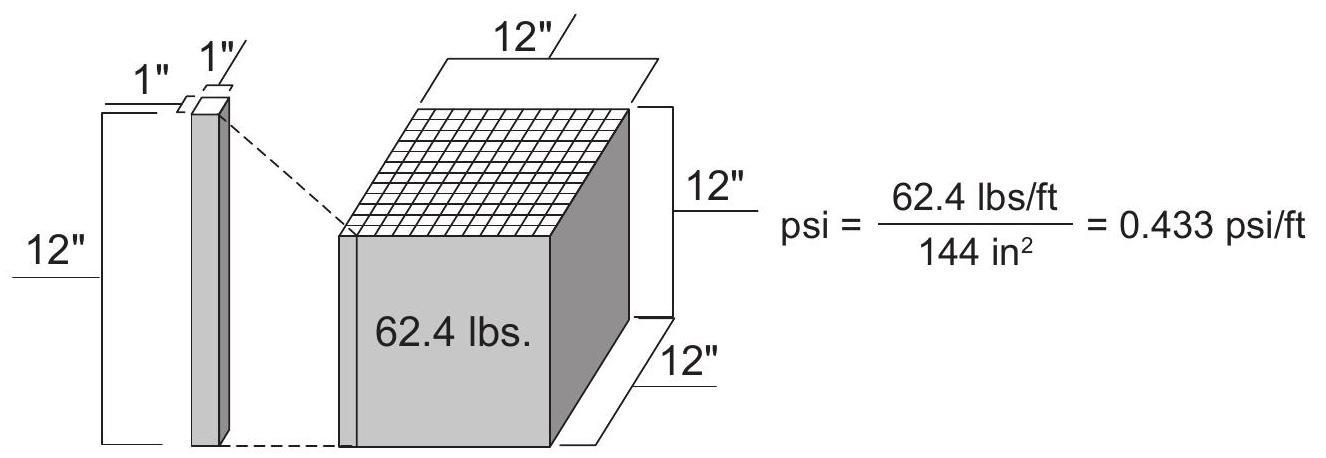
\includegraphics[max width=\textwidth]{2022_11_03_65aa625ded296bdfd01fg-16}

This is the weight of a column of water one inch square and one foot tall. If the column of water were two feet tall and the pressure would be $2 \mathrm{ft}$ x $0.433 \mathrm{psi} / \mathrm{ft}=0.866$ psi.

$1 \mathrm{ft}$ of water $=0.433 \mathrm{psi}$

Conversion feet to psi

With the above information we can convert feet of head ${ }^{31}$ to psi by multiplying the feet of head times $0.433 \mathrm{psi} / \mathrm{ft}$. Example - Conversion feet to $\mathrm{psi}$

A reservoir is 40 feet tall. Find the pressure at the bottom of the reservoir.

$40 \mathrm{ft} \times 0.433 \mathrm{psi} / \mathrm{ft}=17.3 \mathrm{psi}$

Conversion of psi to feet

The conversion of $\mathrm{psi}$ to feet is simply made by dividing the $\mathrm{psi}$ by $0.433 \mathrm{psi} / \mathrm{ft}$.

Example-Conversion of psi to feet

Find the height of water in a tank if the pressure at the bottom of the tank is 12 psi.

$12 \mathrm{psi} \div 0.433 \mathrm{psi} / \mathrm{ft}=27.7 \mathrm{ft}$

\section{Pressure and Head}
Pressure is directly related to the height of a column of fluid. This height is called head or feet of head. From the discussion above we see there is a direct relationship between feet of head and pressure. The relationship is that for every one foot of head there is a pressure of $0.433$ psi.

\section{Pressure Relative to Container Size}
The pressure at the bottom of a container is affected only by the height of water in the container and not by the shape of the container. In the drawing below there are four containers all of different shapes and sizes. The pressure at the bottom of each is the same.

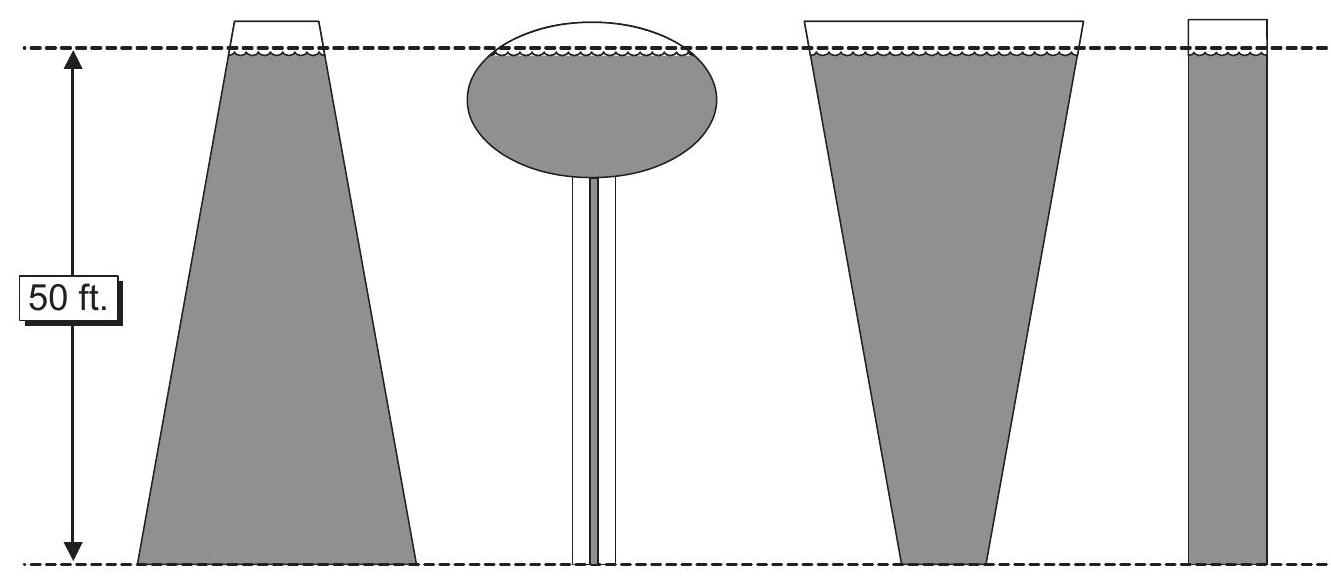
\includegraphics[max width=\textwidth]{2022_11_03_65aa625ded296bdfd01fg-17}

\section{Pressure and Volume}
The pressure exerted at the bottom of a tank is relative only to the head on the tank and not the volume of water in the tank. For example, below are two tanks each containing 5000 gallons. The pressure at the bottom of each is 22 psi. If half of the water were drained from the tanks the pressure at the bottom of the elevated tank would be $17.3$ psi while the pressure at the bottom of the standpipe would be 11 psi.\\

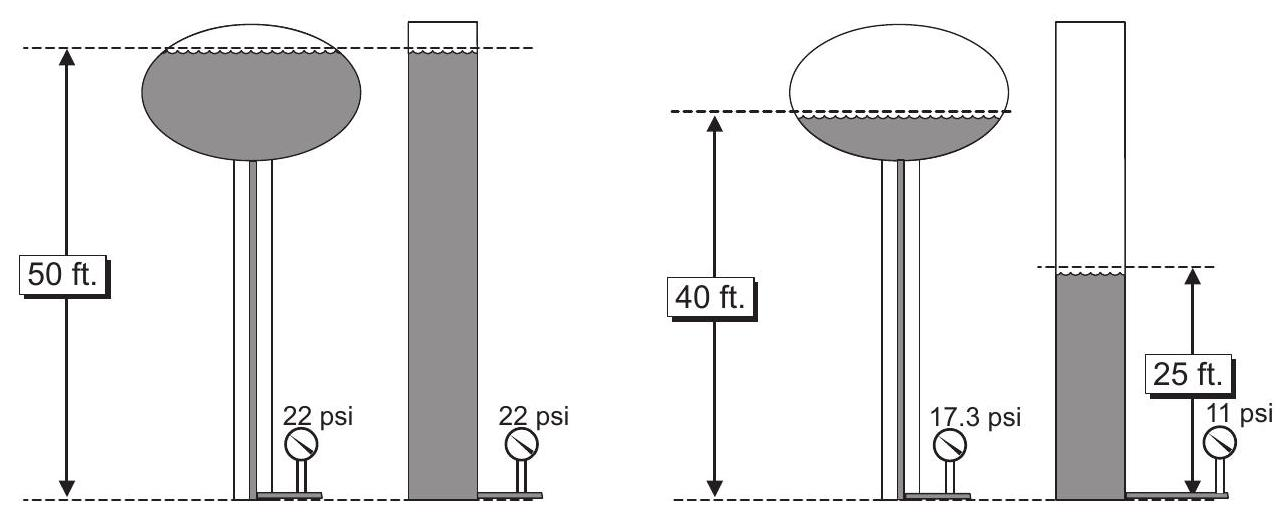
\includegraphics[max width=\textwidth]{2022_11_03_65aa625ded296bdfd01fg-18}

\section{Velocity and Flow}
\section{Velocity}
Velocity is the speed that the water is moving along a pipe or through a basin. Velocity is usually expressed in feet per second, $\mathrm{ft} / \mathrm{sec}$.

\section{Flow}
Flow is commonly expressed in gallons per minute (gpm) and/or cubic feet per second (cfs). There is a relationship between gallons per minute and cubic feet per second. One cubic foot per second is equal to $448.8$ gallons per minute.

$1 \mathrm{cfs}=448.8 \mathrm{gpm}$

\section{Flow Equation}
The basic equation for determining flow is as follows:

$Q=V \times A$

Where:

$\mathrm{Q}=\operatorname{cfs}\left(\mathrm{ft}^{3} / \mathrm{sec}\right)$

$\mathrm{V}=\mathrm{ft} / \mathrm{sec}$

$\mathrm{A}=\mathrm{ft}^{2}$

\section{Static and Dynamic Conditions}
\section{Static Pressure}
${ }^{32}$ Static - A non-moving condition.

The pressure measured when there is no water moving in a line or the pump is not running is called static $^{32}$ pressure. This is the pressure represented by the gauges on the tanks in the discussion above.

\section{Dynamic Pressure}
When water is allowed to run through a pipe and the pressure (called pressure head) measured at various points along the way we find that the pressure decreases the further we are from the sources.

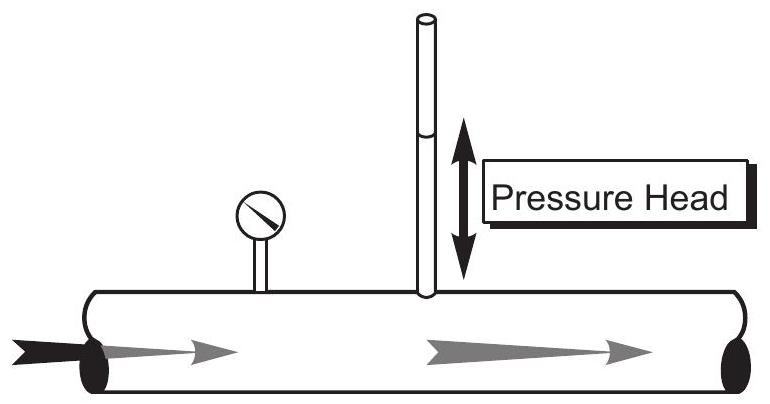
\includegraphics[max width=\textwidth]{2022_11_03_65aa625ded296bdfd01fg-18(1)}

\section{Headloss}
The reason for this reduction in pressure is a phenomenon called headloss. Headloss is the loss of energy (pressure) due to friction. The energy is lost as heat.

\section{Explanation}
When we hear that the headloss in a certain pipe is 25 feet, that means the amount of energy required to overcome the friction in the pipe is equivalent to the amount of energy that would be required to lift this amount of water straight in the air 25 feet.

\section{Factors Contributing to Headloss}
In a pipe, the factors that contribute to headloss include the following:

\begin{itemize}
  \item Roughness of pipe

  \item Length of pipe

  \item Diameter of pipe

  \item Velocity of water

\end{itemize}
\section{Comparison of Factors}
In general, if the roughness of a pipe were doubled the headloss would double. If the length of the pipe were doubled the headloss would double. If the diameter of a pipe were doubled the headloss would be cut in half and if the velocity of the water in a pipe were doubled the headloss would be increased by about four times. It should be apparent that velocity, more than any other single factor, affects headloss. To double the velocity we would have to double the flow in the line.

Example - Headloss

500 feet of four inch line with a flow of $110 \mathrm{gpm}$ has a headloss of $7.5$ feet. At a flow of 220 gpm, the headloss jumps to 26 feet or an increase of $3.5$ times.

\section{Fittings and Headloss}
Each type of fitting has a specific headloss depending upon the velocity of water through the fitting. For instance the headloss though a check valve is two and one quarter times greater than through a ninety degree elbow and ten times greater than the headloss through an open gate valve.

\section{Pumping Hydraulics}
\section{Basic Terms}
\section{Static Head}
Static head is the distance between the suction and discharge water levels when the pump is shut off. Static head conditions are often indicated with the letter $Z$.

\section{Suction Lift}
Suction lift is the distance between the suction water level and the center of the pump impeller. This term is only used when the pump is in a suction lift condition. A pump is said to be in a suction lift condition any time the eye (center) of the impeller is above the water being pumped. ${ }^{33}$ Velocity Head - The amount of energy required to bring a fluid from standstill to its velocity. For a given quantity of flow, the velocity head will vary indirectly with the pipe diameter. ${ }^{34}$ Inertia - The tendency of matter to remain at rest or in motion

${ }^{35}$ Total Dynamic Head (TDH) - The total energy needed to move water from the center line of a pump (eye of the first impeller of a lineshaft turbine) to some given elevation or to develop some given pressure. This includes the static head, velocity head and the headloss due to friction. ${ }^{36}$ Horsepower - A measurement of work, 33,000 foot pounds per minute of work is 1 horsepower.

\section{Suction Head}
Suction head is the distance between the suction water level and the center of the pump impeller when the pump is in a suction head condition. A pump is said to be in a suction head condition any time the eye (center) of the impeller is below the water level being pumped.

\section{Velocity Head}
Velocity head ${ }^{33}$ is the amount of energy required by the pump and motor to overcome inertia ${ }^{34}$ and bring the water up to speed. Velocity head is often shown mathematically as $\mathrm{V}^{2} / 2 \mathrm{~g}$. ( $\mathrm{g}$ is the acceleration due to gravity $-32.2 \mathrm{ft} / \mathrm{sec}^{2}$ ).

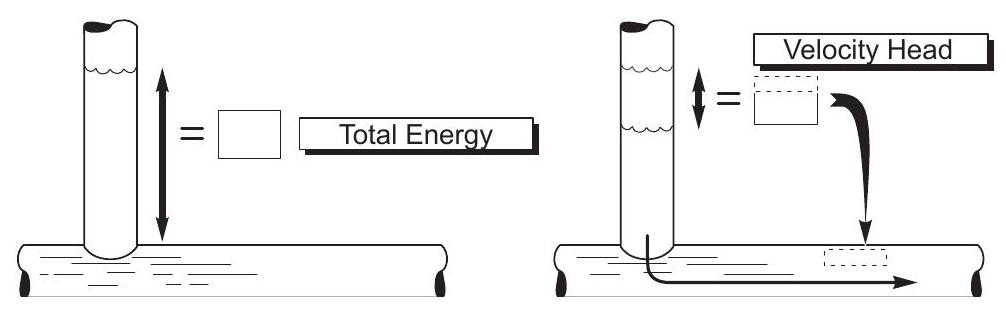
\includegraphics[max width=\textwidth]{2022_11_03_65aa625ded296bdfd01fg-20}

\section{Total Dynamic Head}
Total dynamic head ${ }^{35}$ (TDH) is a theoretical distance. It is the static head, velocity head and headloss required to get the water from one point to another.

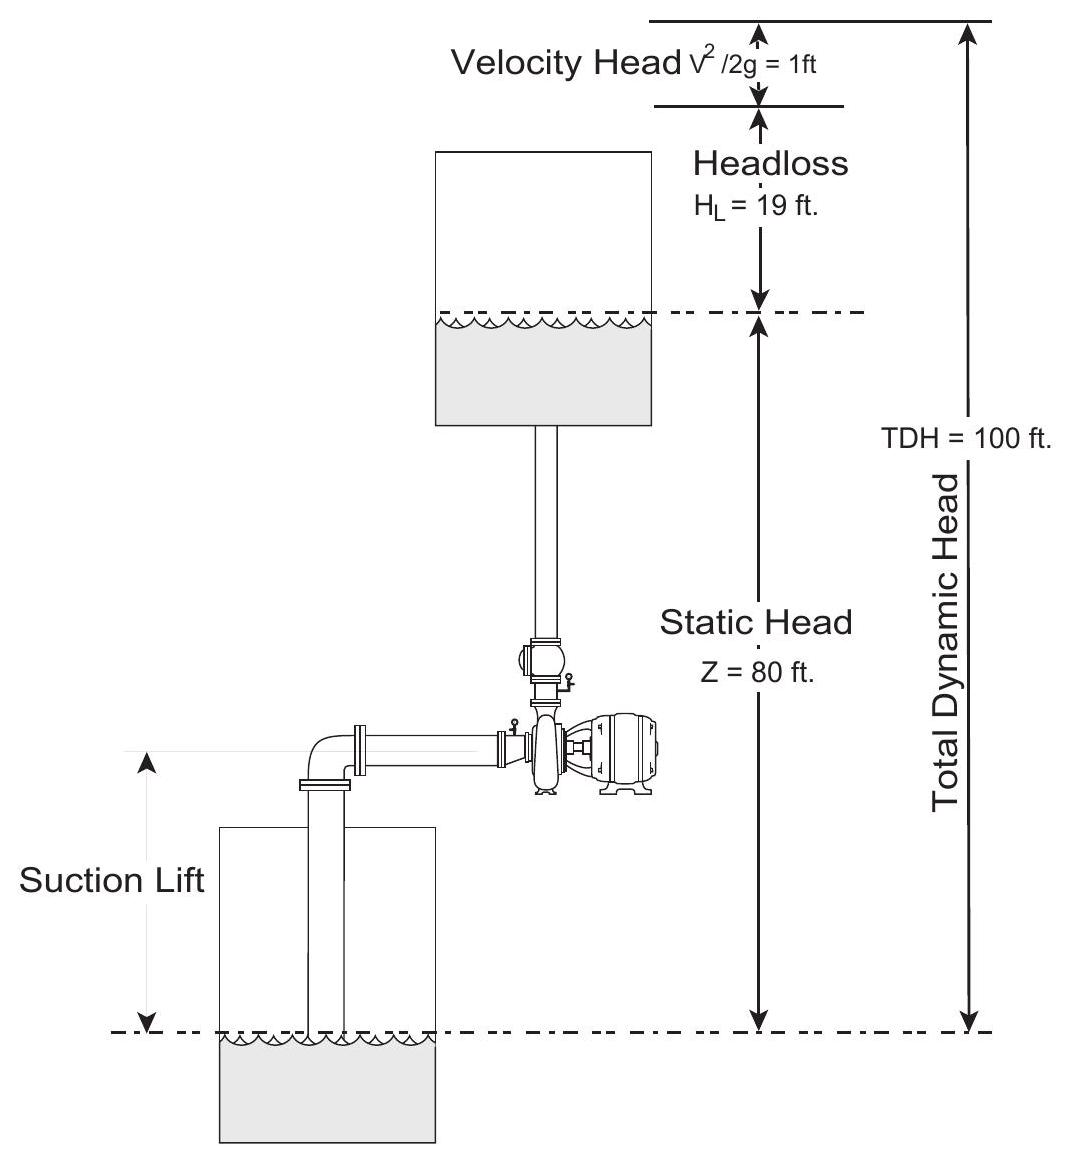
\includegraphics[max width=\textwidth]{2022_11_03_65aa625ded296bdfd01fg-20(1)}

Components of total dynamic head

\section{Horsepower}
Horsepower ${ }^{36}$ is a measurement of the amount of energy required to do work. Motors are rated in horsepower. The horsepower of an electric motor is called brake horsepower. The horsepower requirements of a pump are dependent on the flow and the total dynamic head.

\section{Horsepower and Amperage}
The horsepower output of an electric motor is directly reflected to the amperage ${ }^{37}$ that the motor draws. Any increase in horsepower requirements will give a corresponding increase in amperage.

\section{Pump Response}
For centrifugal pumps, as the total dynamic head is increased the pump will pump less water and will require less horsepower.

\section{Identification}
Identify the components indicated in the drawing below.\\
A. Volute case\\
B. Mechanical seal\\
C. Impeller

${ }^{37}$ Amperage - The measurement of electron flow.

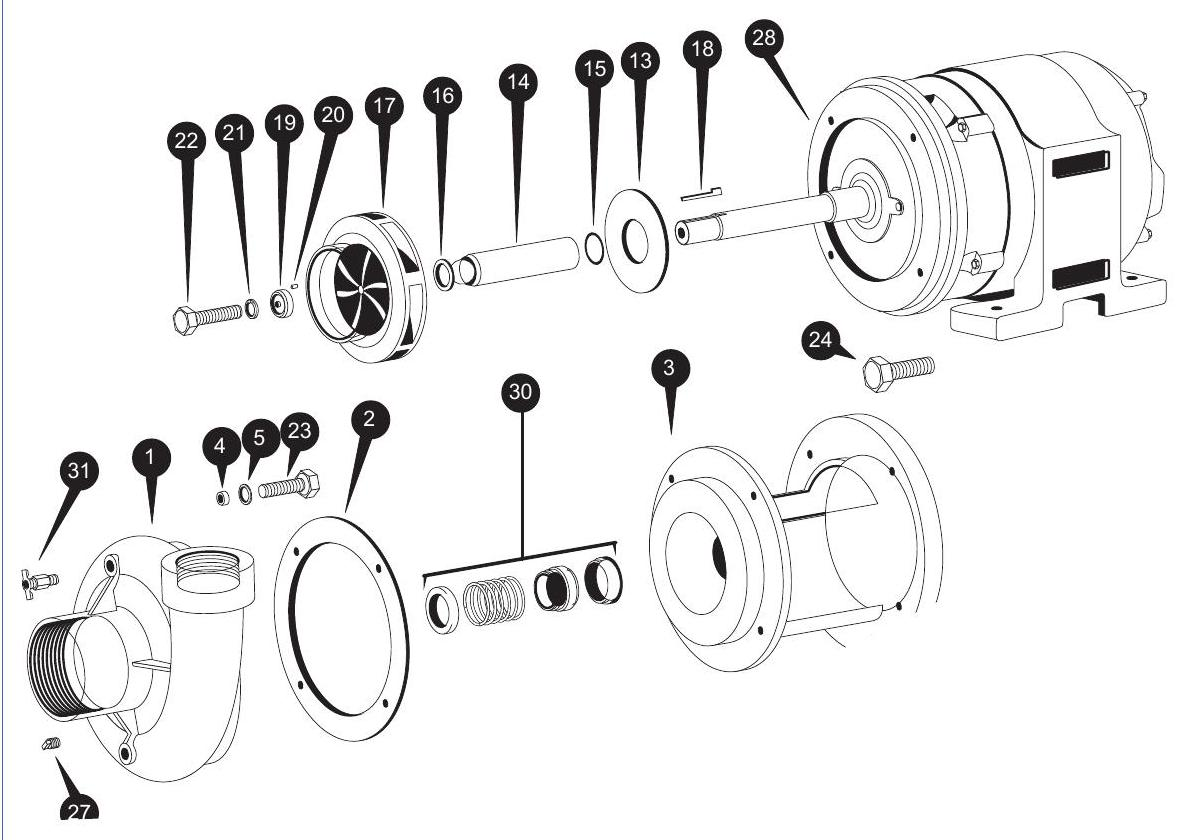
\includegraphics[max width=\textwidth]{2022_11_03_65aa625ded296bdfd01fg-21}

\section{Review}
\begin{enumerate}
  \item One cubic foot of water weighs lons. pounds, and contains gal-

  \item One gallon of water weighs lbs.

  \item Looking at the two reservoirs below, will the pressure at the bottom be:\\
A. The same\\
B. Greater in the tank on the left\\
C. Greater in the tank on the right

\end{enumerate}
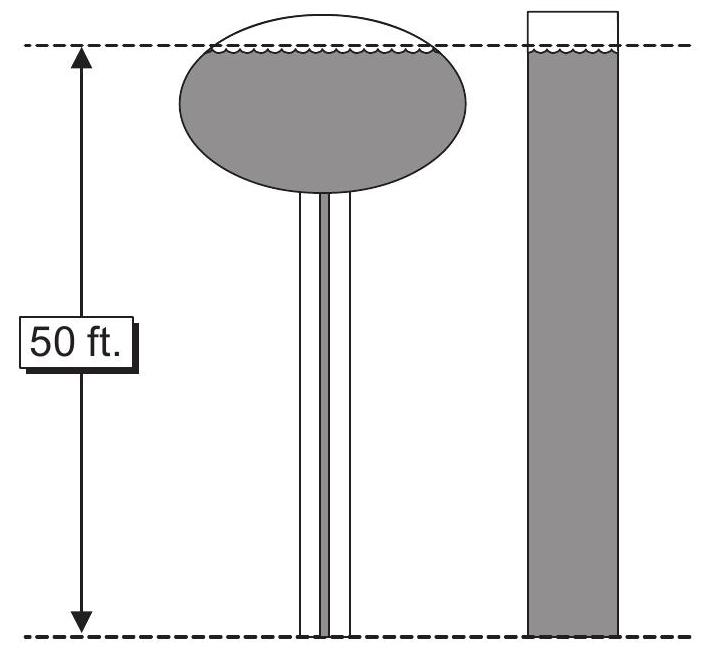
\includegraphics[max width=\textwidth]{2022_11_03_65aa625ded296bdfd01fg-22}

\begin{enumerate}
  \setcounter{enumi}{4}
  \item A tank contains 500 cubic feet. This converts to how many gallons?

  \item A flow of one cubic foot per second is equivalent to gpm.

  \item Headloss is the result of is given off as The energy given off as a result of headloss

  \item What term is used to describe the difference between the level of water in a well and the level of water in the reservoir when the pump is shut down?

  \item What units are used to measure the energy required to do the work of pumping water?

  \item It is 60 feet in elevation from the level of water at the top of the reservoir to the pump house. What is the static water pressure at the pump house?

\end{enumerate}
\section{Identification}
Identify the three pumps below by configuration.

\begin{enumerate}
  \item 
\end{enumerate}
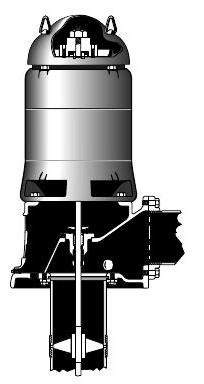
\includegraphics[max width=\textwidth]{2022_11_03_65aa625ded296bdfd01fg-23}

M

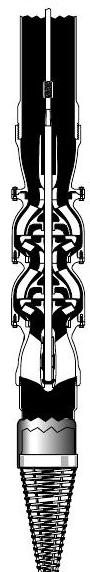
\includegraphics[max width=\textwidth]{2022_11_03_65aa625ded296bdfd01fg-23(1)}

\begin{enumerate}
  \setcounter{enumi}{2}
  \item 
\end{enumerate}
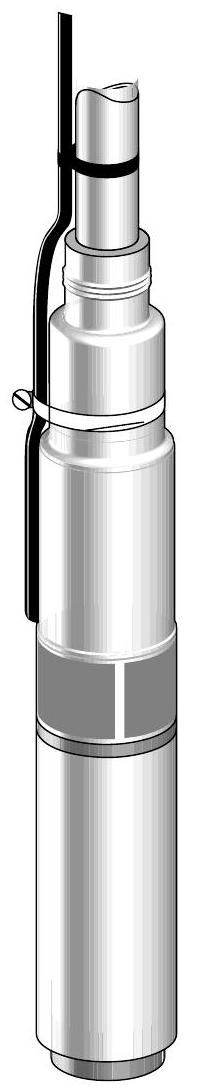
\includegraphics[max width=\textwidth]{2022_11_03_65aa625ded296bdfd01fg-23(2)}

\begin{enumerate}
  \item 
  \item 
  \item 
  \item 
\end{enumerate}
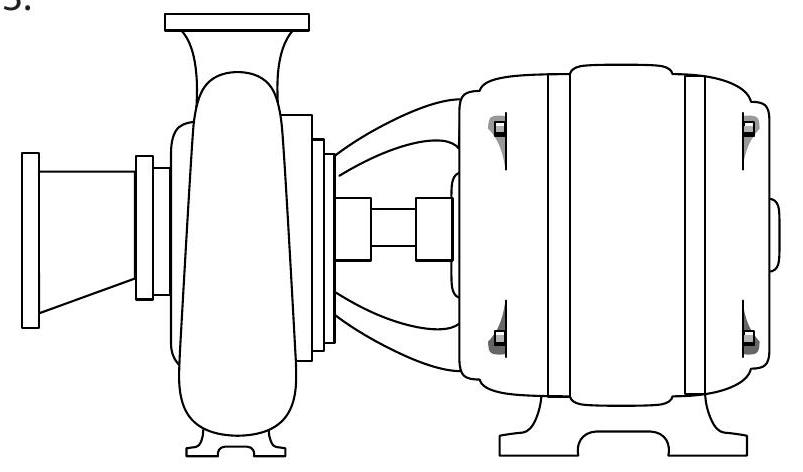
\includegraphics[max width=\textwidth]{2022_11_03_65aa625ded296bdfd01fg-23(3)}

Identify the components indicated in the drawing below.

A.

B.

C.

D.

E.

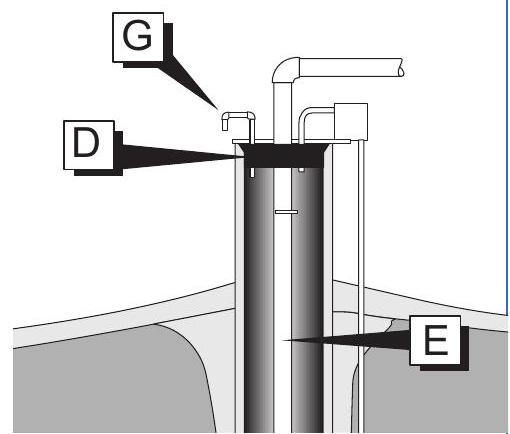
\includegraphics[max width=\textwidth]{2022_11_03_65aa625ded296bdfd01fg-23(4)}

F.

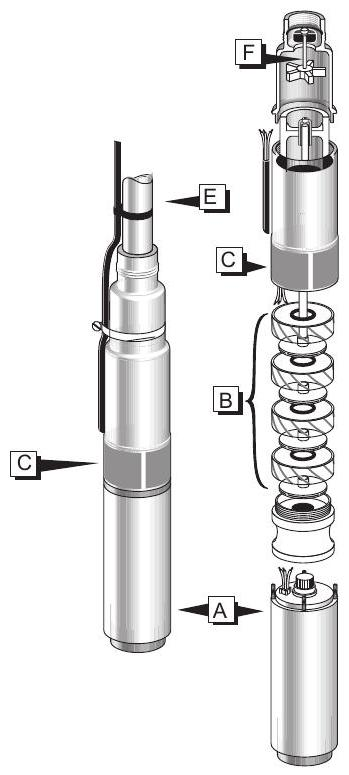
\includegraphics[max width=\textwidth]{2022_11_03_65aa625ded296bdfd01fg-23(5)}

\section{Introduction to Pumping Systems Quiz}
\begin{enumerate}
  \item Which type of pump is frequently used to pump water from wells?\\
A. Progressive cavity pumps\\
B. Submersible turbine pumps\\
C. Reciprocating pumps\\
D. Circulating pumps

  \item What is the purpose of pump mechanical seals?\\
A. Keep leakage off slippery floors\\
B. Prevent leakage between the pump casing and shaft\\
C. Provide an effective backflow prevention device\\
D. Seal water to maintain pump prime

  \item What is the primary purpose of priming a pump?\\
A. Ensure the pump operates freely\\
B. Fill the volute with water\\
C. Prevent backflow\\
D. Start the seal water flow

  \item The component of a centrifugal pump sometimes installed on the end of the suction pipe is called the:\\
A. Volute\\
B. Foot valve\\
C. Impeller\\
D. Packing

  \item Positive displacement pumps should never be operated:\\
A. Backward\\
B. With a closed discharge or suction valve\\
C. Without supervision\\
D. Without a concentric reducer

  \item Pumps that are used to feed chemicals should:\\
A. Never be run in auto\\
B. Never be run dry\\
C. Always be controlled by a flow switch\\
D. Always be controlled by a level sensor

  \item Packing should be adjusted when:\\
A. Excessive leakage from the discharge pipe is noticed\\
B. Excessive leakage from the stuffing box is noticed\\
C. Pump prime is lost\\
D. The pump is shut down 8. Closed impellers should be used for:\\
A. When the pump is used to pump sludge\\
B. When the pump is used to circulate glycol\\
C. When the pump is used to pump chemicals\\
D. When the pump is used to boost pressure

  \item Check valves are used to:\\
A. Control leakage from the stuffing box\\
B. Ensure pump is isolated from the system for maintenance\\
C. Prevent water from flowing in reverse\\
D. Fill water storage tanks

  \item Pump couplings are used to:\\
A. Ensure pump is properly connected to discharge piping\\
B. Connect the motor to the pump\\
C. Provide cooling water for the stuffing box\\
D. Keep the pump primed

  \item One cubic foot of water weighs pounds and contains gallons.\\
A. $8.34 \mathrm{lbs}, 7.48$ gallons\\
B. $7.48 \mathrm{lbs}, 62.4$ gallons\\
C. $11.3 \mathrm{lbs}, 5$ gallons\\
D. $62.4 \mathrm{lbs}, 7.48$ gallons

  \item One gallon of water weighs lbs.\\
A. $3.42 \mathrm{lbs}$\\
B. $7.48 \mathrm{lbs}$\\
C. $8.34 \mathrm{lbs}$\\
D. $4.56 \mathrm{lbs}$

  \item A tank contains 500 cubic feet. This converts to how many gallons?\\
A. 3740 gallons\\
B. $66.8$ gallons\\
C. 4170 gallons\\
D. $59.9$ gallons

  \item A flow of one cubic foot per second is equivalent to\\
A. $62.4$\\
B. $179.5$\\
C. $7.48$\\
D. $448.8$ gpm. 15. Headloss is the result of . The energy given off as a result of headloss is given off as\\
A. Pressure, head\\
B. Friction, heat\\
C. Flow, electricity\\
D. Weight, noise

  \item What term is used to describe the difference between the level of water in a well and the level of water in the reservoir when the pump is shut down?\\
A. Drawdown\\
B. Static head\\
C. Well yield\\
D. Dynamic head

  \item Describe Total Dynamic Head (TDH).\\
A. Total pressure a pump will pump\\
B. Composed of headloss, velocity head, and static head.\\
C. Amount of pressure in a well\\
D. A toilet on a submarine

  \item What is the difference between suction lift and suction head?\\
A. Total dynamic head in the pumping system\\
B. Static head between the pump suction and discharge.\\
C. Relationship between the eye of the impeller of the pump and the surface water from which the pump is pumping.\\
D. There is no difference

  \item What units are used to measure the energy required to do the work of pumping water?\\
A. Microns\\
B. Horsepower\\
C. Foot-pounds\\
D. Gallons per minute

  \item It is 60 feet in elevation from the level of water at the top of the reservoir to the pump house. What is the static water pressure at the pump house?\\
A. $500.4 \mathrm{psi}$\\
B. $25.98 \mathrm{psi}$\\
C. $138.6 \mathrm{psi}$\\
D. $448.8 \mathrm{psi}$

\end{enumerate}

\end{document}